% !TeX spellcheck = <none>
\documentclass[a4paper]{article}
\usepackage[utf8x]{inputenc}
\usepackage{natbib}
\usepackage[francais]{babel}
\usepackage{graphicx}
\usepackage[T1]{fontenc}
\usepackage[left=3cm, right=3cm, top=3cm, bottom=3cm]{geometry}
\usepackage{tikz}
\usepackage{pgfplots}
\usepackage{hyperref}
\usepackage{footnote}
\usepackage{xcolor}
\usepackage{listingsutf8}
\usepackage{verbatim}
\usepackage[bottom]{footmisc}
\usepackage{etoolbox}
%\usepackage{pstricks}
\usepackage{titlesec}
\usepackage{lastpage}

\setcounter{secnumdepth}{4}

\titleformat{\paragraph}
{\normalfont\normalsize\bfseries}{\theparagraph}{1em}{}
\titlespacing*{\paragraph}
{0pt}{3.25ex plus 1ex minus .2ex}{1.5ex plus .2ex}


\usetikzlibrary{patterns}
\pgfplotsset{compat=newest}

\setlength\parindent{0pt}
\setlength{\parskip}{1em}
\lstloadaspects{formats}



% Configure Listings
\definecolor{lightgray}{rgb}{.9,.9,.9}
\definecolor{darkgray}{rgb}{.4,.4,.4}
\definecolor{purple}{rgb}{0.65, 0.12, 0.82}

\lstdefinelanguage{JavaScript}{
	keywords={typeof, new, true, false, catch, function, return, null, catch, switch, var, if, in, while, do, else, case, break},
	keywordstyle=\color{blue}\bfseries,
	ndkeywords={class, export, boolean, throw, implements, import, this},
	ndkeywordstyle=\color{darkgray}\bfseries,
	identifierstyle=\color{black},
	sensitive=false,
	comment=[l]{//},
	morecomment=[s]{/*}{*/},
	commentstyle=\color{purple}\ttfamily,
	stringstyle=\color{red}\ttfamily,
	morestring=[b]',
	morestring=[b]"
}


\lstdefinestyle{Bash}
{language=bash,
	keywordstyle=\color{blue},
	basicstyle=\ttfamily,
	morekeywords={sudo},
	morekeywords={make},
	morekeywords={mkdir},
	morekeywords={cmake},
	morekeywords={python},
	morekeywords={pip},
	morekeywords=[2]{peter@kbpet:},
	keywordstyle=[2]{\color{red}},
	literate={\$}{{\textcolor{red}{\$}}}1 
	{:}{{\textcolor{red}{:}}}1
	{~}{{\textcolor{red}{\textasciitilde}}}1,
}


% Configure Listings
\lstset{
	inputencoding=utf8/latin1,
	basicstyle=\ttfamily,
	stringstyle=\ttfamily\color{green!50!black},
	keywordstyle=\color{blue}\bfseries,
	commentstyle=\color{red!50!black}\itshape,
	showstringspaces=true,
	breaklines=true,
	showspaces=false,
	showstringspaces=false,
	showtabs=true,  
	tabsize=2, frame=single,
	numbers=left, numberstyle=\tiny,
	firstnumber=1, stepnumber=1, numbersep=5pt,	
	moredelim=**[is][\color{red}]{@|}{@|},
	style=Bash,
	captionpos=b,
}


\newtoggle{AbstractOnly}
%\toggletrue{AbstractOnly}
\togglefalse{AbstractOnly}


\newcommand{\fyr}{\emph{Find your ride }}

% Set the docs variables
\title{Rapport \fyr}

\newcommand{\titleA}{\fyr}
\author{Lucien Camuglia}
\newcommand{\enseignants}{M. Zeltner}
\newcommand{\classe}{Classe : T.IS-E2A}
\newcommand{\ecole}{CFPT en informatique}
\newcommand{\formation}{Technicien ES en informatique}
\newcommand{\authorA}{Lucien Camuglia }
\newcommand{\travail}{Travail de diplôme}
\newcommand{\volee}{Session : 2016-2017}
\date{\today}
\newcommand{\rpi}{\emph{Raspbery Pi}}
\newcommand{\rpib}{\emph{Raspbery Pi 3 model B}}
\newcommand{\ocv}{\emph{OpenCV}}
\newcommand{\py}{\emph{Python}}
\newcommand{\gmap}{\emph{Google Maps}}
\newcommand{\bdd}{base de données}
\newcommand{\phpFolder}{../../Includes}
\newcommand{\tabitem}{~~\llap{\textbullet}~~}
\newcommand{\bt}{\emph{boostrap }}


\newcommand{\diag}[1]{\input{../Diagrammes/#1.tex}}
% Save the values
\makeatletter

% mise en page
\usepackage{fancyhdr} 
\pagestyle{fancy} 

%En tete
\renewcommand{\headrulewidth}{1pt}
\fancyhead[L]{\@author}
\fancyhead[R]{\today}
\fancyhead[C]{\fyr}

%Pied de page
\renewcommand{\footrulewidth}{1pt}
\fancyfoot[C]{Page  \thepage / \pageref{LastPage}}
\PassOptionsToPackage{hyphens}{url}\usepackage{hyperref}

% Spacing params
\setlength\parindent{0pt}
\setlength{\parskip}{0.75em}


\begin{document}
\begin{titlepage}
	\centering
	{\LARGE \titleA} \\
	\vspace{1cm}
	{\Large \ecole} \\
	\vspace{0.5cm}
	{\Large \formation} \\
	\vspace{0.5cm}
	{\large \travail}\\
\vspace{1cm}
\begin{figure}[h]
	\centering
	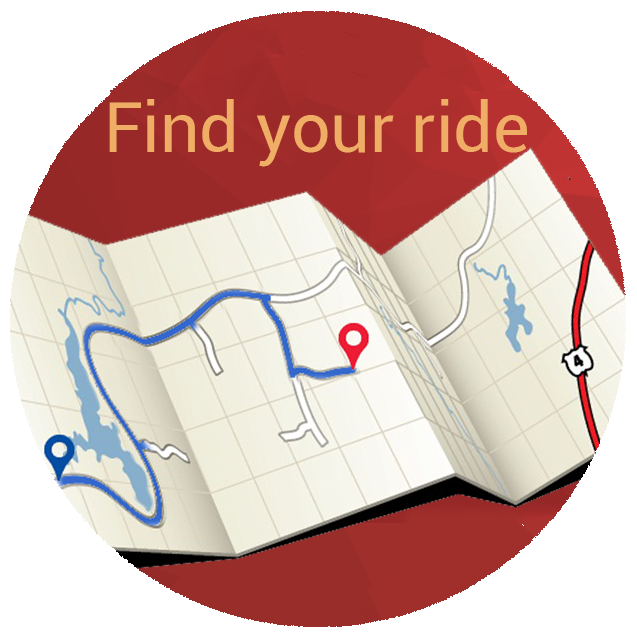
\includegraphics[width=0.9\textwidth]{./Images/logo.png}
\end{figure}

	\vspace{1cm}
	{\large \classe}\\
	\vspace{0.5cm}
	{\large \volee}\\
	\vspace{0.5cm}
	{\large Elève : \hfill Enseignant :}\\
    {\large \authorA  \hfill \enseignants}

	\vfill
% Bottom of the page
	{\large \today\par}
\end{titlepage}
\iftoggle{AbstractOnly}{}
{
\tableofcontents
\pagebreak}


\section{Introduction}
\subsection{Résumé}
Site WEB permettant le partage d'itinéraire entre passionné de la moto.
Ce site est réalisé en HTML/PHP/CSS/AJAX et incluant les API\footnote{\emph{Application Programming Interface}(Interface de Programation Applicative) \url{https://fr.wikipedia.org/wiki/Interface_de_programmation}} Google.

Il permet à un utilisateur de créer un trajet, de le partager et de le modifier.

Un utilisateur peut rechercher un itinéraire avec différents critères :
\begin{itemize}
    \item Durée
    \item Type de route
    \item Changement d'altitude
\end{itemize}

Le site fournit à l'utilisateur différentes données comme le temps du trajet ou la consommation théorique de la moto pour la balade.

Le motard peut aussi importer et exporter des fichiers directement depuis son GPS.


\subsection{Abstract}

The website allows sharing itineraries between motorcycle enthusiasts. The site is set-up with HTML/PHP/CSS/AJAX and Google’s API. It allows users to create trips, to share and modify them.


Different criteria can be defined by the user to create the itinerary:
\begin{itemize}
\item Travel Time
\item Type of road
\item Change in altitude, etc.
\end{itemize}



This website gives the user diverse informations. One example could be the theoretical consumption of their motorcycle for the ride or travel time. The rider can also upload or download files directly from his GPS.



\iftoggle{AbstractOnly}{
\end{document}
}{}
\pagebreak


\section{Cahier des charges}

\subsection{Description}
Site web permettant aux motard de partagé leurs excursions. 

\subsection{But}
Le but de ce travail est d'avoir un site web permettent le partage et la communication entre les passionnés de la moto.

Le site permettra d'afficher sur une carte le tracé du trajet, la durée, leur appréciation personnelle et celle de la communauté, divers commentaire et éventuellement la consommation d'essence.

Le site donnera aussi la possibilité au motard d'importer ou d'exporter des tracés depuis son GPS à l'aide de fichier .GPX

Le tout sera développé autour de l'API Google Map.

\subsection{Spécifications}

\begin{itemize}
	\item Site web réalisé en HTML/CSS/PHP/JS/AJAX
	\item Base de donnée SQL
	\item API Google map
\end{itemize}

\subsection{Restrictions}
\begin{itemize}
	\item Responsive design pour la consultation sur smartphone/tablettes
\end{itemize}



\subsection{Environement}
\begin{itemize}
	\item PC standard de l'école avec droit d'administrateur
	\item Netbeans IDE 7.4
	\item EasyPHP Devserver 7.1.1
\end{itemize}

\subsection{Livrables}
\begin{itemize}
	\item Poster
	\item Dossier d'analyse
	\item CDROM avec les sources
	\item Journal de bord
\end{itemize}

\subsection{Calendrier}
\begin{itemize}
	\item début : mer 05/04/17
	\item reddition intermédiaire (doc + poster) : ven 06/05/17
	\item reddition finale : lun 12/06/17
\end{itemize}


\pagebreak

\section{Analyse de l'existant}


\subsection{Garmin BaseCamp}
Garmin BaseCamp est un logiciel fournit par Garmin.

Il permet à un utilisateur de créer un trajet et de l'importer sur son GPS.

Il donne aussi la possibilités a l'utilisateur de visionner ses différents déplacements.

\begin{tabular}{|l|l|}
	\hline
	Positif                                & Négatif                                       \\ \hline\hline
	\tabitem Connexion directe avec le GPS & \tabitem Pas de partage                       \\
	                                       & \tabitem Obligation de posseder un GPS Garmin \\ \hline
\end{tabular}
 
\subsection{http://www.calculitineraires.fr/}

www.calculitineraires.fr est un site de partage d'itinéraire pour la course à pied, le vélo et la randonnée

Il permet l'import/export de fichier GPX et TCX, la rechercher et le partage d'itinéraire.

\begin{tabular}{|l|l|}
	\hline
	Positif                                   & Négatif                                     \\ \hline\hline
	\tabitem Assez complet                    & \tabitem Interface compliquée d'utilisation \\
	\tabitem Import / Export des fichiers GPS & \tabitem Pas de contribution pour la moto   \\
	\tabitem Création d'itinéraire            &                                             \\ \hline
\end{tabular}


\subsection{http://www.bestbikingroads.com}
www.bestbikingroads.com est un site de partage d'itinéraire moto.


Il permet l'import/export de fichier GPX, la rechercher, le partage d'itinéraire ainsi que la notation des balades.

\begin{tabular}{|l|l|}
	\hline
	Positif                                   & Négatif                                                       \\ \hline\hline
	\tabitem Assez complet                    & \tabitem Tout les tracés s'affiche en meme temps sur la carte \\
	\tabitem Import / Export des fichiers GPS & \tabitem pas de modification possible                         \\
	\tabitem Création d'itinéraire            &                                                               \\
	\tabitem Notation des balades             &                                                               \\ \hline
\end{tabular}

\subsection{Conclusion}
Il existe différent site de partage d'itinéraire, cependant ils ont tous des fonctionnalitées assez similaire. Mon site se distingue des autres de part son interface intuitive pour l'utilisateur et certaines fonctionnalitées trouvée sur aucun site.

Par exemple il est possible sur \fyr de calculer sa consommation théorique pour l'itinéraire ou de filtrer les routes selon leurs sinueusité.



\pagebreak

\section{Analyse fonctionnelle}

\subsection{Généralités}
Ci-dessous se trouve le schéma initial de mon site web. Les ronds représentent des pages et les flèches entre ceux-ci représentent d'éventuelles actions ou états.

\begin{figure}[h]
\centering
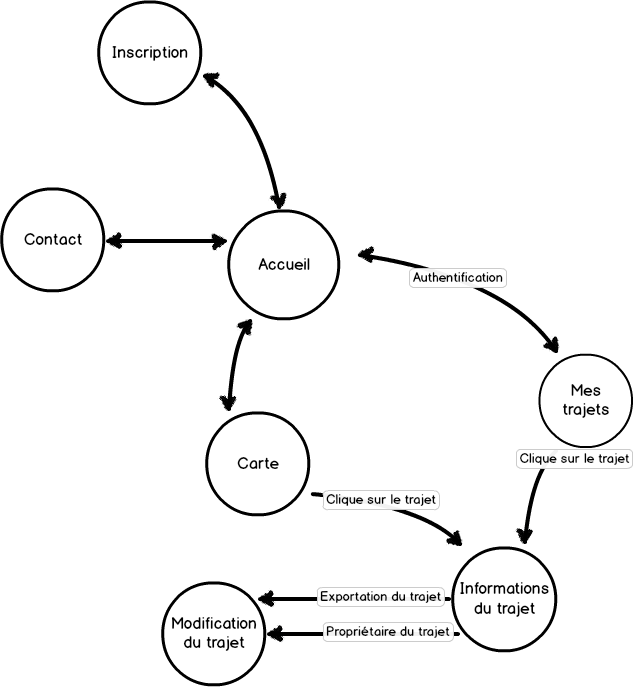
\includegraphics[width=\textwidth]{./Images/ShemaSite.png}
\caption{Schéma du site}
\end{figure}

\subsection{Description des fonctionnalités globales}
\subsubsection{Authentification}
Cette fonctionnalité permet à un utilisateur de s'authentifier et d'accéder à ses trajets mit en ligne ou partager de nouveaux trajets.

\subsubsection{Inscription}
Cette fonctionnalité permet à un nouvel utilisateur de créer un compte et donc de pouvoir bénéficier des fonctionnalités d'un utilisateur connecté

\subsubsection{Création de trajet}
Cette fonctionnalité se distingue en deux sous fonctionnalités : 
\begin{itemize}
    \item Création : crée un nouveau trajet depuis le site directement.
    \item Importation : importe un fichier de type GPX et éventuellement modifier le trajet.
\end{itemize}

\subsubsection{Exportation}
Cette fonctionnalité permet à un utilisateur d'exporter le trajet de son choix au format GPX pour l'inclure dans son GPS.

\subsubsection{Suppression d'un trajet}
Cette fonction permet a un utilisateur de supprimer un de ses trajet.

\subsubsection{Visualiser le trajet}
Cette fonctionnalité permet à n'importe qui de visualiser les trajets mit en ligne, puis les exporter en les modifiant s'il le souhaite.

\subsubsection{Contact}
Cette fonctionnalité permet à n'importe qui de contacter le webmaster afin de faire des remarques ou des demandes.

\newpage

\subsection{Description de l'interface}

\subsubsection{Inscription}
\begin{figure}[h]
\centering
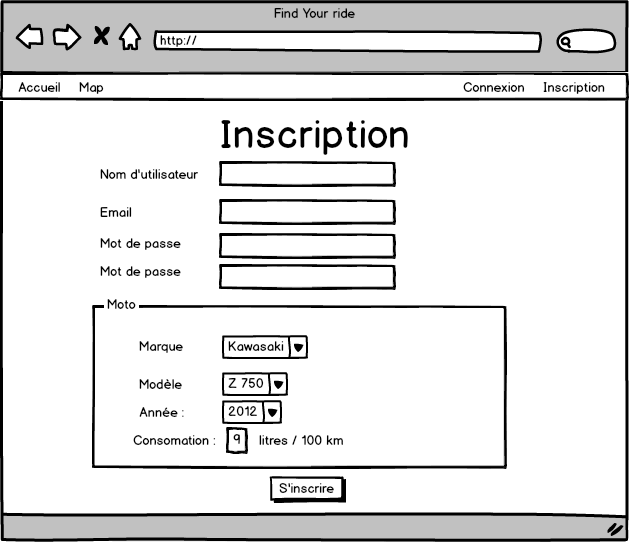
\includegraphics[width=0.5\textwidth]{./Images/Interfaces/inscription.png}
\caption{Page inscription}
\end{figure}

Cette page sert à l'inscription des utilisateurs. On y trouve différent champs : 
\begin{itemize}
    \item Nom d'utilisateur
    \item E-mail
    \item Mot de passe, ce champ apparaît deux fois pour avoir la validation de celui-ci
    \item Moto : diverse informations sur la moto de l'utilisateur comme par exemple sa consomation pour calculer la consomation des trajets.
\end{itemize}

\subsubsection{Map}
\begin{figure}[h]
\centering
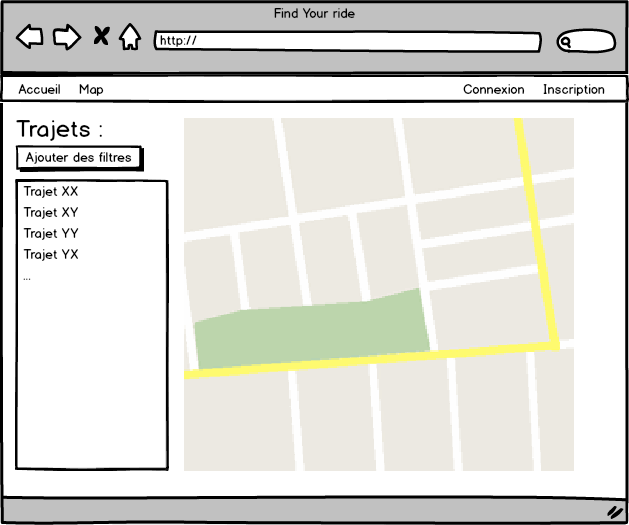
\includegraphics[width=0.5\textwidth]{./Images/Interfaces/Map.png}
\caption{Page inscription}
\end{figure}

Cette page sert à l'affichage de la carte et des différents trajets.

Sur la gauche apparaissent tout les trajets ainsi qu'un bouton filtre.
Ce bouton permet de filtre les trajets parmi différents critères.
\begin{itemize}
    \item Avec ou sans autoroute
    \item Durée
    \item Dénivelé
    %\item sinuosité
\end{itemize}
Sur la droite une carte Google ou apparaît le tracé sélectionné.

\subsubsection{Detail trajet}
\begin{figure}[h]
\centering
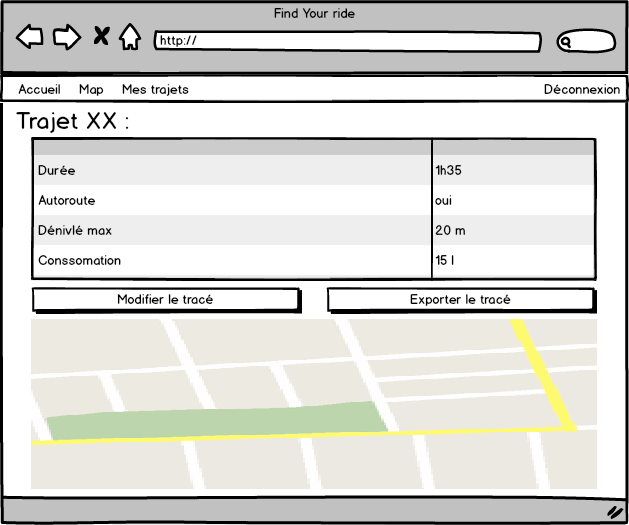
\includegraphics[width=0.5\textwidth]{./Images/Interfaces/DetailTrajet.png}
\caption{Page Detail Trajet}
\end{figure}

Cette page sert à afficher le détail d'un trajet.

Sur le haut de la page apparai les détails du trajet.
\begin{itemize}
    \item Durée du trajet
    \item S'il contient des autoroutes
    \item Dénivelé
    \item La consomation (si l'utilisateur à renseignée les données de la moto)
    %\item sinuosité
\end{itemize}
Deux bouton sont présent pour modifier ou exporter le trajet.
Sur le bas de la page, la carte google avec le trajet.

\subsubsection{Connexion}
\begin{figure}[h]
\centering
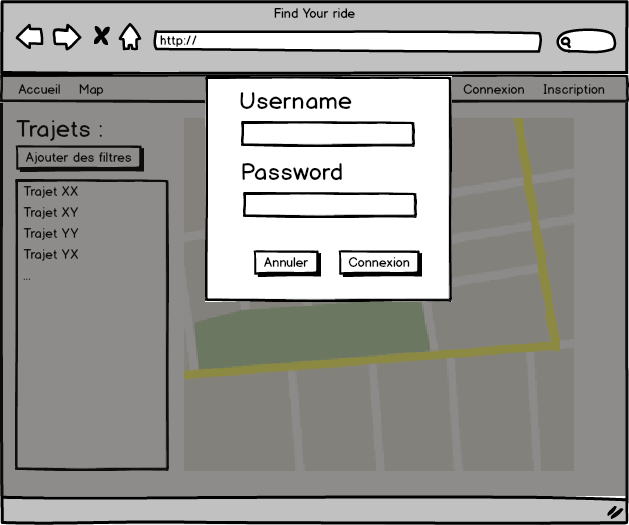
\includegraphics[width=0.5\textwidth]{./Images/Interfaces/Connexin.png}
\caption{Modal connexion}
\end{figure}

Le formulaire de connexion est une fenêtre modal qui s'ouvre par dessus les autres pages avec uniquement deux champs.
\begin{itemize}
    \item Nom d'utilisateur
    \item Mot de passe
\end{itemize}


\subsubsection{Vos trajets}
\begin{figure}[h]
\centering
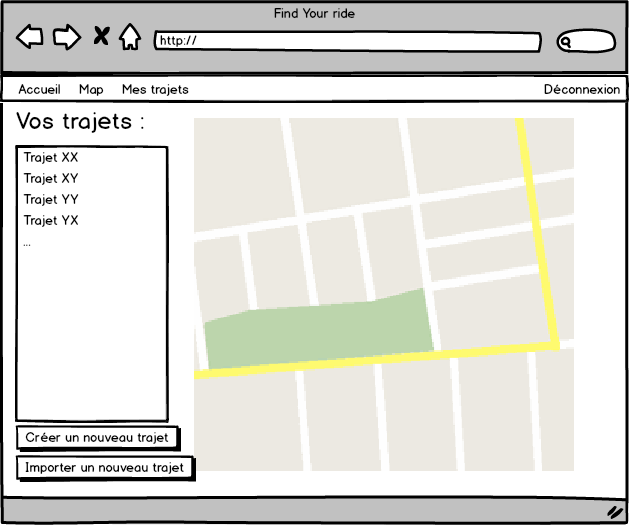
\includegraphics[width=0.5\textwidth]{./Images/Interfaces/VosTrajets.png}
\caption{Page vos trajet}
\end{figure}

Cette page est identique que la page \emph{Map} mais au lieu d'avoir tout les trajet disponible du site, il y a uniquement les trajet de l'utilisateur.

Deux boutons sont disponible sur cette page.
\begin{itemize}
    \item Créer un nouveau trajet, permet de créer un trajet a partir de la carte
    \item Importer un nouveau trajet, permet d'importer un fichier GPX avec le trajet.
\end{itemize}

\subsection{Description des éléments de sécurité}
\subsubsection{Fichier .htaccess}
Permet d'empêcher la navigation sur certain dossier/fichiers du site. Ils permettent aussi de définir des pages d'erreurs personnalisées

\subsubsection{Utilisateur de la base de données}
Utiliser un utilisateur différent que \emph{root} pour accéder à la base de donnée afin de donner des droits qu'au éléments nécessaire.

\subsubsection{Requêtes}
Utilisation de requêtes préparée pour éviter les injections SQL.


\pagebreak








\pagebreak


\section{Analyse organique} 
\subsection{Résumé}
Dans cette section sera expliqué le fonctionnement de l'application.

\subsection{\emph{Boostrap}}
N'étant pas designeur web j'ai décidé de réaliser le design du site à l'aide du framework\footnote{Infrastrucuture de devloppement. \url{https://fr.wikipedia.org/wiki/Framework}} \bt.

Le framework \bt initialement appelé \emph{Twitter Blueprint} à été créé en 2010 par \emph{Twitter}.

Il offre une collection d'outils d'aide à la création du design d'un site web.

L'avantage de cet outil est la compatibilité avec les versions récentes des navigateurs, il est aussi \emph{responsive} ce qui permet la consultation du site sur tout types d'écran, que ce soit oridnateur, tablette ou smartphone.



\subsection{Google API}
Les API\footnote{\emph{Application Programming Interface}(Interface de Programation Applicative) \url{https://fr.wikipedia.org/wiki/Interface_de_programmation}} Google sont une suite d'outils développé et fourni par Google pour permettre à des utilisateurs d'intégrer les services Google dans un site web ou une application.

Il en existe environ 66 dont 16 pour \gmap. Pour la réalisation de ce site j'utilise 4 API \gmap : 
\begin{itemize}
    \item Google Maps Javascript
    \item Google Direction
    \item Google Elevation
    \item Google Roads
\end{itemize}

\subsubsection{Google Maps Javascipt}
Cette API permet d'intégrer une \gmap \ sur le site web, c'est la seule qui sera visible pour l'utilisateur. C'est sur celle-ci qu'apparaissent les itinéraires et les positions GPS.
\subsubsection{Google Direction}
Le fonctionnement de cette API est assez simple. Il suffit d'envoyer un point d'origine et une destination à Google Direction et il nous retourne un tableau JSON avec différent paramètres.
\begin{itemize}
    \item La durée
    \item La distance
    \item Les étapes du parcours (positions GPS)
    \item Les étapes du parcours (Francais, par exemple : Tournez a droite,...)
\end{itemize}

\subsubsection{Google Elevation}
Cette API permet d'obtenir l'altitude de points géographique à la surface de la Terre, y compris les fonds marins.

Les données géographique peuvent être fournie de deux façon différente : 
\begin{itemize}
	\item En tant que point géographique
	\item En tant que tracé
\end{itemize}

Pour mon site l'utilisation sera faite à l'aide de tracé afin d'avoir les altitudes de chaque point de la route.


\subsubsection{Google Roads}
Cette API permet de faire 3 choses différentes :
\begin{itemize}
    \item \emph{Snap to raod}
    \item \emph{Nearest road}
    \item \emph{Speed limits}
\end{itemize}

J'utilise deux fonctionnalitées de cette API, \emph{Snap to raod} et \emph{Nearest road}.

\emph{Snap to raod} permet de "déplacer" un trajet pour qu'il suive la route. Il faut lui envoyer l'ensemble des point GPS de notre route et il nous retourne un ensemble de point qui suivent la route.

\emph{Nearest road} permet de donner la position d'un point GPS sur la route la plus proche.

\subsection{Fichier GPX}
GPX est un format de fichier ouvert permettant l'échange de coordonée GPS. Il peut contenir trois types d'informations : 

\begin{itemize}
	\item Point de cheminement (\emph{waypoint})
	\item Route
	\item Trace
\end{itemize}

Le fichier suit la même structure que le XML.

Ci dessous, un exemple de fichier GPX

\begin{lstlisting}[frame=single] 
<?xml version="1.0" encoding="UTF-8"?>
<gpx version="1.0" creator="FindYourRide.org" xmlns:xsi="http://www.w3.org/2001/XMLSchema-instance" xmlns="http://www.topografix.com/GPX/1/0" xsi:schemaLocation="http://www.topografix.com/GPX/1/0 http://www.topografix.com/GPX/1/0/gpx.xsd">

<trk>
<name>Journal actif: 2016-06-28 15:47</name>
<trkseg>
<trkpt lat="46.188097" lon="6.196411">
<ele>397.64</ele>
<time>2016-06-28T14:47:33Z</time>
<extensions>
<gpxtpx:TrackPointExtension>
<gpxtpx:course>0.00</gpxtpx:course>
</gpxtpx:TrackPointExtension>
</extensions>
</trkseg>
</trkpt>
</trk>

\end{lstlisting}


\subsection{Fonction PHP pour la \bdd}
\subsubsection{connexion à la \bdd}
La connexion à la \bdd se fait à l'aide de PDO\footnote{\emph{PHP Data Object}, \url{http://php.net/manual/fr/intro.pdo.php}}. PDO a besoin de l'utilisateur de la \bdd et du mot de passe ainsi que le nom de la base.
Je lui précise aussi le mode d'erreur qui est \emph{PDO::ERRMODE\_EXCEPTION} ce mode permet d'afficher le code d'erreur et de déclencher une exception\footnote{Plus d'informations \url{http://php.net/manual/fr/pdo.error-handling.php}}.

Afin d'avoir un partage d'informations dans le bon format, on défini l'encodage de caractères en UTF-8

\subsubsection{Requêtes préparées}
Afin de sécuriser le site et éviter les injections SQL j'utilise des requêtes préparées.

On commence par préparer la requête, PDO va substituer les marqueurs (\emph{:marqueur}) pour les valeur fournie dans le tableau de paramètres fourni au moment de l'exécution. Ensuite, il faut exécuter la requête avec les parametres.

\subsubsection{GetMotorcycleBrand}
Ne prend pas de paramètre d'entrée.

Récupère dans la base de données toutes les marques de moto.

Retourne un tableau contenant les marques.
\subsubsection{GetMotorcycleModel}
Ne prend pas de paramètre d'entrée.

Récupère dans la base de donées tout les models de moto.

Retourne un tableau contenant les models trié par ordre alphabétique.
\subsubsection{GetAllMotorcycleYear}
Ne prend pas de paramètre d'entrée.

Récupère dans la base de données toutes les années.

Retourne un tableau contenant les années dans l'ordre croissant.
\subsubsection{GetAllMotorcycleConsumption}
Ne prend pas de paramètre d'entrée.

Récupère dans la base de données toutes les consommations.

Retourne un tableau contenant les consommations dans l'ordre croissant.
\subsubsection{GetAllMotorcycleTiredness}
Ne prend pas de paramètre d'entrée.

Récupère dans la base de données touts les indices de fatigue.

Retourne un tableau contenant les indices de fatigue dans l'ordre croissant.
\subsubsection{GetAllMotorcycles}
Ne prend pas de paramètre d'entrée.

Récupère dans la base de données toutes les motos.

Retourne un tableau contenant toutes les motos et leurs informations trié par marque. 
\subsubsection{GetRoutes}
Prend un paramètre facultatif qui est l'identifiant de l'utilisateur.

Récupère dans la base de données les routes. Soit toutes les routes, soit les route de l'utilisateur.

Retourne un tableau contenant les routes.

\subsubsection{CreateRoute}
Prend 3 données en entré, le nom de la route, l'identifiant de l'utilisateur et si la route contient des autoroutes.

Insère les données dans la base de données

Retourne l'identifiant de la route créée.

\subsubsection{deletePlaces}
Prend entrée l'identifiant de la route.

Supprime touts les points GPS de la route dans la base de données.

Ne retourne rien

\subsubsection{addPlaceToRoute}
Prend en entrée 4 paramètres, la latitude, la longitude, la position du point dans le tracé et l'identifiant de la route.

Insère les informations dans la base de données.

Ne retourne rien

\subsubsection{deleteMotorcycle}
Prend en entrée l'identifiant de la moto

Supprime la moto

Ne retourne rien.

\subsubsection{getUserNMotorcycle}
Ne prend pas de paramètre d'entrée.

Récupère toutes les infomrations d'un utilisateur et de sa moto.

Retourne un tableau avec toutes les informations.


\subsubsection{getUserRoleById}
Prend en entrée l'identifiant de l'utilisateur.

Selectionne dans la \bdd le role de l'utilisateur.

Retourne le rôle.

\subsubsection{AddSinuosity}
Prend en entrée l'identifiant de la route et la sinueusité.

Ajoute la sinueusité dans la \bdd

Ne retourne rien.

\subsubsection{AddElevation}
Prend en entrée l'identifiant de la route et l'altitude.

Ajoute l'altitude dans la \bdd

Ne retourne rien.

\subsubsection{AddLength}
Prend en entrée l'identifiant de la route et la longueure.

Ajoute la longueure dans la \bdd

Ne retourne rien

\subsubsection{GetmostSinuousRoad}
Ne prend rien en entrée.

Sélectionne dans la \bdd \ la route la plus sinueuse.

Retourne la valeur de la route la plus sinueuse.

\subsubsection{GetLessSinuousRoad}
Ne prend rien en entrée.

Sélectionne dans la \bdd \ la route la moins sinueuse.

Retourne la valeur de la route la moins sinueuse.

\subsubsection{GetMostSteepestRoad}
Ne prend rien en entrée.

Sélectionne dans la \bdd \  la route la plus "pentue".

Retourne la valeur de la route la plus "pentue".

\subsubsection{GetLessSteepestRoad}
Ne prend rien en entrée.

Sélectionne dans la \bdd \  la route la moins "pentue".

Retourne la valeur de la route la moins "pentue".

\newpage
\subsection{Inscription sur le site}

Afin de pouvoir bénéficier de toutes les fonctionnalitées du site, l'utilisateur doit se connecter. Si celui-ci n'a pas de compte, il a la possibilité d'un créer un. 

La création d'un utilisateur se fait en plusieurs étapes :
\begin{itemize}
    \item Contrôle en AJAX lors de la saisie des informations par l'utilisateur
    \item Contrôle en PHP des informations
    \item Création de l'utilisateur en PHP et SQL
\end{itemize}

La vérification Ajax est assez simple, lorsque l'utilisateur appuye sur une touche, on affiche une croix rouge puis on envoie une requete à la page PHP qu va nous retourner un booléen a \emph{true} si l'utilisateur exite. S'il est vrai, on laisse la croix rouge sinon on affiche un vu vers.

Une fois la verification faite en javascript/ajax, les données sont envoyées a une fonction PHP qui revérifie si l'utilisateur est déjà présent dans la base, puis, récupère l'identifiant de la moto daprès la marque, le model et l'année.
Finalement, les données sont ajoutée à la base de données.
\begin{center}
	 \diag{Inscription}
\end{center}




\subsection{Connexion au site}
Une fois l'inscirption effectuée, l'utilisateur a la possibilité de se connecter au site.

Pour ce faire, l'utilisateur saisi ses informations dans le formulaire et se connecte.
Une première vérification en HTML5 vérifie que les champs soient remplis(\emph{required}).
Une fois cette vérification éffectuée, les informations sont envoyée à la page PHP \emph{connexion.php} qui vérifie encore une fois que les champs soient rempli. Puis, envoie les données à la fonction PHP de connexion qui va récupérer :
\begin{itemize}
	\item Les ids utilisateur
	\item Les mots de passe
	\item Les roles
\end{itemize}

Une fois ces informations récupérée, on les parcour tous pour être sûr que le nom d'utilisateur et le mot de passe fourni correspondent bien à un utilisateur existant.
Si c'est le cas, on enregistre l'id, le role et le nom d'utilisateur dans des \emph{Sessions} et on retourne \emph{true} pour dire que les informations sont correcte.

\begin{center}
	\diag{Connexion}
\end{center}

\subsection{\emph{Upload} d'un itinéraire}
L'utilisateur à la possibilité de mettre en ligne ses itinéraires depuis un fichier \emph{.GPX}.

Premierement, un script vérifie l'extension du fichier. Une fois l'extension vérifiée, une fonction enregistre chaque point du fichier dans la \bdd. Finalement, une fonction javascript envoie a google les point et récupère la position sur la route (API Google Roads) et enregistre les nouvelles coordonées.

\begin{center}
	\diag{Gpx2Sql}
\end{center}


\subsection{Téléchargement d'un itinéraire}
Un itinéraire disponnible sur le site est téléchargeable.
Pour ce faire, l'utilisateur choisi l'itinéraire et clique sur \emph{Download route}.

Le traitement se fait en PHP.

Le trajet et le nom sont transmit à la fonction qui va  vérifier si un fichier du même nom existe déja. Si c'est le cas, le fichier est supprimé et un autre est créé. 

On ajoute ensuite l'entête du fichier XML et GPX.

\lstset{language=XML}
\begin{lstlisting}[frame=single] 
<?xml version="1.0" encoding="UTF-8"?>
<gpx version="1.0" creator="FindYourRide.org" xmlns:xsi="http://www.w3.org/2001/XMLSchema-instance" xmlns="http://www.topografix.com/GPX/1/0" xsi:schemaLocation="http://www.topografix.com/GPX/1/0 http://www.topografix.com/GPX/1/0/gpx.xsd">
\end{lstlisting}

Une fois ces informations insérée dans le fichier il faut ajouter le nom, chaque point et fermer les balises.

\begin{center}
	\diag{PathToGpx}
\end{center}


\subsection{Fonction javascript de gestion de la carte}
Ci-dessous sont toutes les fontions utilisée pour créer et gérer la carte Google.

\subsubsection{Initialisation de la carte}
L'initialisation de la carte se fait à plusieurs moment : 
\begin{itemize}
	\item Chargement de la page
	\item Chargement d'un itinéraire
	\item Modification d'un intinéraire
\end{itemize}

Lors de l'appel de l'initalisation il faut définir deux choses :
\begin{itemize}
	\item Si le trajet peut être modifié
	\item Si le trafic doit être affiché
\end{itemize}

Par défaut la carte est centrée sur Genève. Si La géolocalisation est disponible et activée sur le navigateur, la carte se centre sur le lieu de l'utilisateur.

Si la variable de modification est vrai, un évenemment \emph{click} sera ajouté à la carte.

De plus, si l'utilisateur choisi de visualiser le traffique en temps réel, un calque avec le traffique sera rejouté a \gmap


\begin{center}
	\diag{initMap}
	\caption{initmap}
\end{center}

\subsubsection{ImportGPX}
Prend en paramètre le fichier GPX à importer.

Fait un appel AJAX à la méthode d'import de fichier.

Ne retourne rien.

\subsubsection{AskGoogle}
Prend en paramètre le chemin de la route.

Fait un appel AJAX à l'API Google \emph{snapToRoads}.

Récupère chaque valeures données par l'API.

Retourne un tableau avec ces nouvelles valeures.

\subsubsection{LoadPoints}
Prend en paramètre l'identifiant de la route.

Fait un appel AJAX à la fonction \emph{GetRoutePoints}.

Récupère chaque valeur dans un tableau.

Retourne le tableau .

\subsubsection{SnappPoints2Road}
Prend en paramètre la route (sous fomrat d'un tableau de points).

Parcour le tableau et toute les 50 positions, appel la fonction \emph{AskGoogle}

Retourne un tableau avec toutes le postions.

\subsubsection{SaveNewLocation}
Prend 3 paramètres, l'identifiant de la route, la route (sous fomrat d'un tableau de points), et un boolean pour savoir si la route vien depuis l'API google.

\begin{center}
\diag{SaveNewRoute}
\end{center}

\subsubsection{CreateRoute}
Prend 2 paramètres, le nom de la route et si elle contient des autoroutes.

Vérifie que le nom ne soit pas vide.

Fait un appel AJAX à la fonction \emph{CreateRoute}.

Appel \emph{SaveNewLocation} avec les valeurs reçu.

Ne retourne rien.

\subsubsection{RouteClick}
Ne prend pas de paramètres.
Ajoute un événement click sur tout les objets contenant la classe \emph{route}.

Cet événement comprend :

Effacer les informations sur la carte.

Initialiser la carte sans modification.

Défini l'action du bouton \emph{DeleteRoute} par la suppression de la route sélectionnée.

Enlève l'attribut \emph{hidden} du bouton de modification du tracé.

Enlève l'attribut \emph{hidden} des objects ayant pour classe \emph{routeControl}.

Modifie l'attribut \emph{name} du bouton \emph{btnModif}.

Retire la classe \emph{highlighted} de la route en surbriance.

Ajoute la classe \emph{highlighted} à la route actuelle.

Défini la variable \emph{highlighted} avec cet objet.

Appel \emph{ShowParcour}.

Appel \emph{DisplayRouteInfo}.

ne retourne rien 

\subsubsection{searchIti}
Prend en paramètre 2 tableaux de point GPS, le premier contient le lieu d'origine et le second contient la destination.

Crée une varialbe contenant la requête de recherche (origine, destination, mode de voyage, autoroutes?).

Défini la carte dans le servcie \emph{Direction} de \emph{Google}.

Cherche la route.

Ajoute chaque étape de la route dans la variable globale \emph{route}.

Affiche la route.

Ne retourne rien.

\subsubsection{Clear}
Ne prend pas de paramètre.

Efface la tableau de marqueur.

Efface le tableau contenant la route.

Ne retroune rien.

\subsubsection{ShowParcours}
Prend en paramètre le tableau de points GPS du tracé, si le parcour peut etre modifier et la couleur du parcour.

Si la couleur n'est pas définie, défini la couleur par défaut (\#ff1ece).

Si le tracé peut être modifié, appel \emph{CreateMarker} pour le marqueur de début et fin.

Ajout au tableau \emph{route} les point du tracé.

Etand les "bornes" pour centrer la carte sur la totalité du tracé.

Appel la fonction \emph{DisplayRoute}.

\subsubsection{DisplayRoute}
Prend en paramètre la couleur du tracé.

Si aucun paramètre n'est saisi, défini la couleur avec la couleur par défaut (\#ff1ece).

Affiche la \emph{Polyline} du tracé sur la carte.

ne retourne rien.

\subsubsection{CreateMarker}
Prend en paramètre, la localisation du marqueur, si la parcour peut etre modifié, si le marqueur peut etre supprimé, la couleur du marqueur, le texte du marquer et sa position (ordre du tracé).

Défini l'image du marquer selon la couleur et le texte choisi.

Crée le marqueur.

Si la marqueur peut etre supprimé, ajoute les évenements de suppréssion.

si le marqueur peut etre modifié, ajoute les évenements de modification.

Ajute le marqueur au tableau de marqueurs.

Ne retourne rien.

\subsubsection{refreshValues}
Cette fonction sert à raffrachir la valeur d'un point GPS dans les zones de saisie.

\subsubsection{DownloadRoute}
Ne prend pas de paramètres.

Vérifie qu'un itinéraire soit sélectionné.

Récupère le nom de l'itinéraire.

Fait un appel AJAX à la fonction PHP \emph{Download} avec comme paramètres, le nom de la route et le chemin.

Fait appel à la page de téléchargement avec le nom du fichier.

ne retourne rien.

\subsubsection{EnableDisabledFilters}
Prend en paramètre le checkbox.

Vérifie si le checkbox est checker ou non.

Ajoute ou retire l'attribut \emph{Hidden}.

Si les filtre doivent être affiché, appel \emph{RefreshRouteWithFilters} sinon appel \emph{RefreshRouteWithoutFilters}.

\subsubsection{RefreshRouteWithFilters}
Ne prend pas de paramètres.

Récupère la valeur de tout les filtres. (sinueusité, Pente et autoroute).

Fait un appel AJAX à la fonction PHP \emph{FilterRoad} avec comme paramètres les valeurs récupérée précédement.

Supprime l'affichage de toutes les routes. 

Ajoute chaque route que l'AJAX nous a retourné.

Appel la fonction \emph{RouteClick}

Ne retourne rien.

\subsubsection{RefreshRouteWithoutFilters}
Ne prend pas de paramètres.

Fait un appel AJAX à la fontion PHP \emph{GetRoutes}

Supprime l'affichage de toutes les routes.

Ajoutes les routes que l'AJAX nous a retourné.

Appel la fonction \emph{RouteClick}.

Ne retourne rien.

\subsubsection{StartCreation}
Ne prend pas de paramètres.

Appel la fonction \emph{ClearRoute}.

Enlève la classe CSS \emph{Hidden} à tout les objets qui ont pour classe \emph{SaveRouteControls}.


\subsubsection{DisplayRouteInfo}
Prend en paramètre l'identifiant de la route.

Fait un appel AJAX à la fonction PHP \emph{GetRoadsInfos}.

Affiche toutes les informations retournée par l'appel AJAX dans les champs prévu à cet effet.

Ne retourne rien.

\subsubsection{DeleteRoute}
Prend en paramètre l'identifiant de la route.

Fait un appel AJAX à la fonction PHP \emph{DeleteRoute}.

Recharge la page.


\subsubsection{ClearRoute}
Ne prend pas de paramètre.

Appel la fonction \emph{InitMap}

Vide tout les tableaux de données.

\subsubsection{Document.Ready}
Appel la fonction \emph{initMap}.

Appel la fonction \emph{Clear}.

Appel la fonction \emph{RouteClick}.

Ajoute un événement click sur le bouton \emph{btnmodif}.

Ajoute un événement click sur le bouton \emph{RefreshRoute}.

Ajoute un événement lorsque la valeur du \emph{slider} de sinueusité change.

Ajoute un événement lorsque la valeur du \emph{slider} d'altitude change.

Ajoute un événement lorsque la case a cocher du filtre d'autoroute change.

Ajoute un événement click sur le bouton \emph{StartCreation}.

Ajoute un événement click sur le bouton \emph{ClearRoute}.

Ajoute un événement lorsque la case a cocher d'utilisation des autoroute change.

\subsubsection{Document.bind}
Ajoute une classe \emph{loading} au body lorsque une requête AJAX démarre.

Retire la classe \emph{loading} au body lorsque une requête AJAX se termine.

Ce système permet d'afficher une roue qui tourne pour faire patienter l'utilisateur.

\subsection{fonction javascript pour l'inscription et la connexion}
\subsubsection{connexion}
Prend un paramètre qui est un tableau contenant l'utilisateur et le mot de passe.

Fait un appel AJAX à la page PHP \emph{Connexion}.

Vérifie la réponse AJAX et recharge la page ou affiche un message d'erreur.

ne retourne rien 

\subsubsection{LoadModalFromBrand}
Prend en paramètre la marque.

Fait un appel AJAX à la fonction PHP \emph{GetModel}

Affiche tout les model retourné par l'AJAX.

Ne retourne rien.

\subsubsection{LoadYearFromModel}
Prend 2 paramètres, la marque et le model.

Fait un appel AJAX à la fonction PHP \emph{GetYear}

Affiche toutes les années retournée par l'AJAX.

Ne retourne rien.

\subsubsection{UserNameExists}
Prend en paramètre le nom d'utilisateur.

Crée une variable existe a faux.

Fait un appel AJAX à la fonction PHP \emph{UserExists}.

Défini a vrai la variable si l'utilisateur existe.

Retourne la variable.

\subsubsection{checkForEnabled}
Ne prend pas de paramètre.

Vérifie pour chaque champs de saisie s'il y a la croix rouge. Si c'est la cas, desactive le bouton submit.

Ne retourne rien.

\subsubsection{Document.Ready}
Active les info-bulles.

Pour chaque champ de saisie, active le contrôle de saisie et mets a jour la croix rouge ou le vu vert.


\subsection{Fonction ajax}

\subsubsection{GetModel}
Prend en entrée la marque.

Sélectionne dans la \bdd touts les model correspondant à la marque.

Retourne un tableau JSON contenant touts les models.

\subsubsection{GetYear}	
Prend en entrée la marque et le model.

Sélectionne dans la \bdd toutes les années d'un véhicule.

Retourne un tableau JSON contenant toutes les années.

\subsubsection{UserExists}
Prend en entrée le nom d'utilisateur.

Sélectionne dans la \bdd l'utilisateur contenant ce nom d'utilisateur.

Si la \bdd retourne quelquechose, retourne vrai sinon retourne faux


\subsubsection{GetMotorcycles}
Prend en entrée marque, model, année, consomation et indice de fatigue.

Sélectionne dans la \bdd les motos correspondant aux critères saisis.

Retourne un tableau contenant toutes les informations des motos.

\subsubsection{GetRoutePoints}
Prend en entrée l'identifiant de la route.

Sélectionne dans la \bdd tout les points GPS correspondant à l'identifiant de la route.

retourne un tableau contenant touts les points

\subsubsection{SaveNewRoute}
Prend en entrée l'identifiant de la route, la route, la sinueusité, l'altitude et la longugeure.

Supprime les points enregistré pour cette route.

Ajoute la sinueusité.

Ajoute l'altitude.

Ajoute la longueure.

Vérifie le format d'entrée de la route, si c'est un string, le convertit en tableau.

Pour chaque points de la route, appel la méthode d'ajout du point.

Ne retourne rien.

\subsubsection{AddMotorcycle}
Prend en entrée, la marque, le model, l'année, la consomation et l'indice de fatigue.

Vérifie que les champs ne soient pas nul.

Ajoute la moto dans la \bdd.

Retourne un tableau conteant soit un message d'erreur soit rien du tout.

\subsubsection{UpdateUserRole}
Prend en entrée, l'identifiant d'utilisateur et l'identifiant du futur rôle.

Vérifie que l'utilisateur connecté est administrateur.

Met à jours le rôle de l'utilisateur.

Retourne un tableau contenant soit une erreur soit le nouveau rôle de l'utilisateur.

\subsubsection{GetUserRole}
Prend en entrée, l'identifiant de l'utilisateur.

Appel la méthode GetUserRoleById.

Retourne le nom du rôle.

\subsubsection{downloadRoute}
Prend en entrée, le nom de la route et sont parcour.

Appel la fonction "Path2Gpx".

Retourne le nom du fichier.

\subsubsection{FilterRoad}
Prend en entrée tout les paramètres d'une route (sinueusité, pente, autoroute, durée).

Sélectionne dans la \bdd les routes qui correspondent aux critères saisi en entrée.

Retourne un tableau JSON avec toute les données.


\subsubsection{GetRoutesJSON}
Ne prend aucun paramètre.

Récupères toutes les routes en appelant la fonction \emph{GetRoutes}.

Retourne les routes au format JSON.


\subsubsection{GetRoadsInfos}
Prend enentrée l'identifiant de la route.

Récupère dans la \bdd les informations de la route et, si l'utilisateur est connecté, récupère la consommation de sa moto.

Retourne un tableau JSON avec les informations.

\subsubsection{CreateNewRoute}
Prend en entrée le nom de la nouvelle route ainsi que si elle contient des autoroutes.

Appel la méthode CreateRoute.

Retourne l'identifiant de la nouvelle route au format JSON.

\subsubsection{DeleteRoute}
Prend en paramètre l'identifiant de la route.

Supprime dans la \bdd les lieu comportant l'identifiant de la route ainsi que la route.

Retourne "Success" au format JSON
\newpage
\subsection{Base de données}
La moteur de \bdd \ utilisé est \emph{l'InnoDB}, afin de garder les valeur en \emph{UTF-8}.
Le système de gestion de la \bdd est \emph{MySQL}.

\subsubsection{Modèle conceptuel}
\begin{figure}[h]
	\centering
	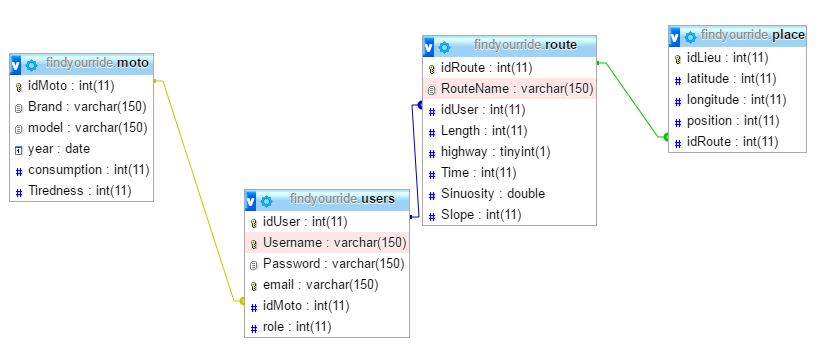
\includegraphics[width=\textwidth]{./Images/MCD.png}
	\caption{Modèle conceptuel de données}
\end{figure}

\subsubsection{Structure de la \bdd}
\paragraph{Table \emph{moto}}
Cette table regroupe toutes les motos du site.

\begin{tabular}{|l|l|l|}
	\hline
	Colone          & Type         & Description                  \\ \hline\hline
	\textbf{idMoto} & int          & Identifiant de la moto       \\ \hline
	Brand           & Varchar(150) & Marque de la moto            \\ \hline
	model           & Varchar(150) & Modèle de la moto            \\ \hline
	year            & date         & Date de sortie de la moto    \\ \hline
	consumption     & int          & Consommation de la moto      \\ \hline
	Tiredness       & int          & Indice de fatigue de la moto \\ \hline
\end{tabular}

\paragraph{Table \emph{users}}
Cette table regroupe touts les utilisateurs du site.

\begin{tabular}{|l|l|l|}
	\hline
	Colone          & Type         & Description                  \\ \hline\hline
	\textbf{iduser} & int & Identifiant de l'utilisateur \\ \hline
	Username & Varchar(150) & Nom de l'utilisateur \\ \hline
	Password & Varchar(150) & Mot de passe de l'utilisateur (sha1) \\ \hline
	email & Varchar(150) & E-mail de l'utilisateur \\ \hline
	\#idMoto & int & Identifiant de la moto \\ \hline
	role & int & Role de l'utilisateur \\ \hline
\end{tabular}

\paragraph{Table \emph{route}}
Cette table regroupe toutes les routes du site.

\begin{tabular}{|l|l|l|}
	\hline
	Colone          & Type         & Description                  \\ \hline\hline
	\textbf{idRoute}& int & Identifiant de la route \\ \hline
	RouteName & Varchar(150) & Nom de la route \\ \hline
	\#idUser & int & Identifiant de l'utilisateur créateur de la route \\ \hline
	Length & int & Longueur de la route (en mètres) \\ \hline
	Highway & Tinyint & La route contient des autoroutes ? \\ \hline
	Time & int & Durée de la route \\ \hline
	Sinuosity & double & Sinueusité de la route \\ \hline
	Slope & double & Pente moyenne de la route \\ \hline
\end{tabular}

\paragraph{Table \emph{Place}}
Cette table regroupe touts les points géographique du site.

\begin{tabular}{|l|l|l|}
	\hline
	Colone          & Type         & Description                  \\ \hline\hline
	\textbf{idLieu} & int & Identifiant du lieu \\ \hline
	latitude & double & Latitude de l'endroit \\ \hline
	longitude & double & Longitude de l'endroit \\ \hline
	position & int& position dans le traçé \\ \hline
	\#idRoute & int & Identifiant de la route correspondante au lieu \\ \hline
\end{tabular}
\pagebreak



\section{Estimation de l'apport personnel}
\begin{tabular}{|l|p{11cm}|c|}
	\hline
	Fichiers & Détails & pourcentage \\ \hline \hline
	*.php & J'ai réalisé la totalité des pages PHP & 100\% \\ \hline
	*.css & J'ai réalisé une partie du code CSS nécéssaire pour le positionnement de certain objet sinon le reste est fait par \emph{bootstrap} & 5\% \\ \hline
	*.js &J'ai réaliser la totalité des fontion de gestion pour google map ormis les fonctions d'affichage des lignes modifiable. Le reste des fichier sont ceux de \emph{bootstrap} et je ne les ai pas modifié &80\% \\ \hline
\end{tabular}

\newpage
\section{Problèmes rencontré}
\subsection{Google Api}
Durant ce projet, j'ai été confronté à l'utilisation des API Google. 

Ces API sont bien doccumentée et il est facile de comprendre comment les utiliser.

Cependant Google a établi des quotas assez stricte ce qui fait qu'on se retrouve vite limité.

Il m'est arrivé a plusieures reprise de ne plus pouvoir faire de requête car j'avais atteint le nombre maximal de requête. 

Pour remedier à ce problème, j'ai créé plusieurs compte devloppeur Google et lorsque l'un de mes compte arrivais à la limite des quotas je changeais de clef d'API.

Cette méthode n'est néanmois pas optimal et il n'est pas possible de publier un site web dans ces conditions.

La solution est de payer un abonement auprès de Google afin d'obtenir plus de requête journalière.
\subsection{Asynchrone}
Les fonctions de rappel javascript fonctionnent toutes de façon asynchrone.

J'ignorais  cet aspect au début du travail, ce qui fait qu'il m'a fallut un peu de temps pour comprendre pourquoi certaine variables changeais de valeur "toute seule" ou avait des valeurs différente en mode deboguage.

Pour l'AJAX, lorque j'avais besoin qu'une fonction de rappel ne soit pas asynchrone, j'utilisait le champ \emph{async} que je définissait a \emph{false}.

\newpage
\section{Conclusion}
\subsection{Bilan personnel}
Durant ce projet de 9 semaines, j'ai pu découvrir les outils de dévloppement Google. Ceux-ci sont très complet et rélativement simple d'utilisation grâce à leurs bonne documentation. 

Je regrette de ne pas avoir fait un bon planning dès le début car je me suis perdu arrivé à environ la moitié du projet. Une bonne plannification m'aurais permis de travailler plus efficacement en suivant un fil conducteur.

L'objectif de mon travail qui était \emph{"avoir un site web permettent le partage entre les passionnés de la moto"} est atteint.
\subsection{Améliorations }
Au fur et à messure du travil des idées me sont apparue pour l'amélioration du site :
\begin{itemize}
	\item Permettre aux utilisateur de noter un itinéraire.
	\item Fournir à l'utilisateur un lien unique pour partager un itinéraire avec des personnes externe au site.
	\item Permettre à l'utilisateur d'avoir plusieurs moto et de les gérer
	\item Ajouter la "fatigue" sur les itinéraires
\end{itemize}

\pagebreak



\listoffigures

\end{document}